%%%%%%%%%%%%%%%%%%%%%%%%%%%%%%%%%%%%%%%%%%%%%%%%%%%%%%%%%%%%%%%%%%%%%%%%%%%%%
%% 03_arch_bus_concept.tex -- Variant A (RV_NoPipeline)
%% Wishbone B4 Classic only. Shared parts: 03_arch_bus_wishbone,
%% 03_arch_bus_slavebpi (spec_common/03_arch).
%%%%%%%%%%%%%%%%%%%%%%%%%%%%%%%%%%%%%%%%%%%%%%%%%%%%%%%%%%%%%%%%%%%%%%%%%%%%%

%%%%%%%%%%%%%%%%%%%%%%%%%%%%%%%%%%%%%%%%%%%%%%%%%%%%%%%%%%%%%%%%%%%%%%%%%%%%%
\subsection{Overview}
%%%%%%%%%%%%%%%%%%%%%%%%%%%%%%%%%%%%%%%%%%%%%%%%%%%%%%%%%%%%%%%%%%%%%%%%%%%%%

Variant~A has one on-chip data bus, \textbf{Wishbone B4 Classic}.
The CPU is the only master. The slaves are D-Mem, GPIO0, CGU, UART0 and ICU0
(Table~\ref{tab:sysmap}).
The instruction memory is not on Wishbone; the CPU reads it through a
separate flat instruction bus (\texttt{iBusAddr\_o}, \texttt{iBusDataRd\_i}).
There is no cache and no AXI4 bus.

%%%%%%%%%%%%%%%%%%%%%%%%%%%%%%%%%%%%%%%%%%%%%%%%%%%%%%%%%%%%%%%%%%%%%%%%%%%%%
\subsection{Wishbone B4 Classic -- Peripheral Bus}
%%%%%%%%%%%%%%%%%%%%%%%%%%%%%%%%%%%%%%%%%%%%%%%%%%%%%%%%%%%%%%%%%%%%%%%%%%%%%

\subsubsection{Signal Naming Convention}

Wishbone signal names in this design follow the convention shown in
Table~\ref{tab:asBusConcept02}.
The suffix \texttt{\_i} indicates an input, \texttt{\_o} an output,
and \texttt{\_s} an internal wire.
The prefix \texttt{wb\_s\_} is used for slave-side signals and
\texttt{wb\_m\_} for master-side signals.

\begin{table}[H]
\caption{Wishbone Signal Naming}
\label{tab:asBusConcept02}
\centering
\begin{tabularx}{\textwidth}{|l |l |l |l |X|}
  \hline
  Wishbone Name & Slave Port & Master Port & Width & Description \\
  \hline
  \hline
  ADR    & \texttt{wb\_s\_addr\_i} & \texttt{wb\_m\_addr\_o} & 64 & Address bus \\
  \hline
  DAT\_I & \texttt{wb\_s\_dat\_i}  & \texttt{wb\_m\_dat\_i}  & 64 & Data from master to slave (write data) \\
  \hline
  DAT\_O & \texttt{wb\_s\_dat\_o}  & \texttt{wb\_m\_dat\_o}  & 64 & Data from slave to master (read data) \\
  \hline
  WE     & \texttt{wb\_s\_we\_i}   & \texttt{wb\_m\_we\_o}   & 1  & Write enable: 1 = write, 0 = read \\
  \hline
  SEL    & \texttt{wb\_s\_sel\_i}  & \texttt{wb\_m\_sel\_o}  & 8  & Byte select (all bytes must be set) \\
  \hline
  STB    & \texttt{wb\_s\_stb\_i}  & \texttt{wb\_m\_stb\_o}  & 1  & Strobe: valid cycle indicator from master \\
  \hline
  ACK    & \texttt{wb\_s\_ack\_o}  & \texttt{wb\_m\_ack\_i}  & 1  & Acknowledge: normal end of transfer from slave \\
  \hline
  CYC    & \texttt{wb\_s\_cyc\_i}  & \texttt{wb\_m\_cyc\_o}  & 1  & Cycle: bus cycle active (held for complete transfer) \\
  \hline
\end{tabularx}
\end{table}

\subsubsection{Transfer Protocol}

A Wishbone Classic single transfer proceeds as follows:

\begin{enumerate}
  \item The master asserts \texttt{CYC} and \texttt{STB}, presents a valid
    address on \texttt{ADR}, drives \texttt{WE} (1 for write, 0 for read),
    sets \texttt{SEL} to all-ones, and -- for a write -- provides data on
    \texttt{DAT\_O}.
  \item In this implementation the slave responds \emph{combinatorially} in the
    same clock cycle: it drives read data on \texttt{DAT\_O} and asserts
    \texttt{ACK}.
  \item The transaction is complete when both \texttt{STB} and \texttt{ACK}
    are seen high on the rising clock edge.
    The master may then begin a new transfer in the very next cycle.
\end{enumerate}

A transfer is considered valid only when both \texttt{CYC} and \texttt{STB}
are asserted simultaneously and all byte-select bits are set.
If any byte-select bit is clear the BPI treats the access as invalid and
suppresses both the ACK and the write enable to the peripheral.

The timing diagram below illustrates a write followed by a read.

\begin{figure}[H]
\centering
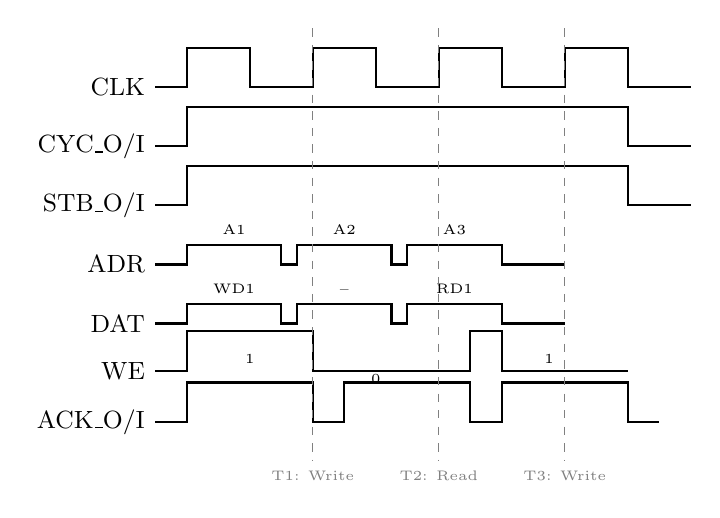
\begin{tikzpicture}[x=0.8cm, y=0.5cm]
  % Clock
  \draw[thick] (0,8) node[left]{\small CLK}
    -- ++(0.5,0) -- ++(0,1) -- ++(1,0) -- ++(0,-1) -- ++(1,0) -- ++(0,1) -- ++(1,0) -- ++(0,-1)
    -- ++(1,0) -- ++(0,1) -- ++(1,0) -- ++(0,-1) -- ++(1,0) -- ++(0,1) -- ++(1,0) -- ++(0,-1) -- ++(1,0);
  % CYC
  \draw[thick] (0,6.5) node[left]{\small CYC\_O/I}
    -- ++(0.5,0) -- ++(0,1) -- ++(7,0) -- ++(0,-1) -- ++(1,0);
  % STB
  \draw[thick] (0,5) node[left]{\small STB\_O/I}
    -- ++(0.5,0) -- ++(0,1) -- ++(7,0) -- ++(0,-1) -- ++(1,0);
  % ADR (two phases)
  \draw[thick] (0,3.5) node[left]{\small ADR}
    -- ++(0.5,0)
    -- ++(0,0.5) -- ++(1.5,0) node[midway,above]{\tiny A1}
    -- ++(0,-0.5) -- ++(0.25,0) -- ++(0,0.5)
    -- ++(1.5,0) node[midway,above]{\tiny A2}
    -- ++(0,-0.5) -- ++(0.25,0) -- ++(0,0.5)
    -- ++(1.5,0) node[midway,above]{\tiny A3}
    -- ++(0,-0.5) -- ++(1,0);
  % DAT (write, then read)
  \draw[thick] (0,2) node[left]{\small DAT}
    -- ++(0.5,0)
    -- ++(0,0.5) -- ++(1.5,0) node[midway,above]{\tiny WD1}
    -- ++(0,-0.5) -- ++(0.25,0) -- ++(0,0.5)
    -- ++(1.5,0) node[midway,above]{\tiny --}
    -- ++(0,-0.5) -- ++(0.25,0) -- ++(0,0.5)
    -- ++(1.5,0) node[midway,above]{\tiny RD1}
    -- ++(0,-0.5) -- ++(1,0);
  % WE
  \draw[thick] (0,0.8) node[left]{\small WE}
    -- ++(0.5,0) -- ++(0,1) -- ++(2,0) -- ++(0,-1) -- ++(2.5,0) -- ++(0,1) -- ++(0.5,0) -- ++(0,-1)  -- ++(2,0);
  \node at (1.5,1.1)  {\tiny 1};
  \node at (3.5,0.6)  {\tiny 0};
  \node at (6.25,1.1) {\tiny 1};
  % ACK
  \draw[thick] (0,-0.5) node[left]{\small ACK\_O/I}
    -- ++(0.5,0) -- ++(0,1) -- ++(2,0) -- ++(0,-1)
    -- ++(0.5,0) -- ++(0,1) -- ++(2,0) -- ++(0,-1)
    -- ++(0.5,0) -- ++(0,1) -- ++(2,0) -- ++(0,-1) -- ++(0.5,0);
  % Labels
  \draw[dashed,gray] (2.5,9.5) -- (2.5,-1.5) node[below]{\tiny T1: Write};
  \draw[dashed,gray] (4.5,9.5) -- (4.5,-1.5) node[below]{\tiny T2: Read};
  \draw[dashed,gray] (6.5,9.5) -- (6.5,-1.5) node[below]{\tiny T3: Write};
\end{tikzpicture}
\caption{Wishbone Classic Single Transfers: Write -- Read -- Write}
\label{fig:asBusTiming01}
\end{figure}

\subsubsection{Byte Select}

The 8-bit \texttt{SEL} signal indicates which byte lanes carry valid data.
Bit\;$n$ of \texttt{SEL} corresponds to byte lane\;$n$ (bits $8n+7\ldots 8n$)
of the 64-bit data bus.
In the current implementation, the master BPI always drives all eight
\texttt{SEL} bits to~1 (full-word transfers only).
The slave BPI checks that all \texttt{SEL} bits are set before asserting
\texttt{ACK} or issuing a write enable to the peripheral kernel.
Sub-word accesses are therefore not supported.

\subsubsection{Reset Behaviour}
\label{subsubsec:wbResetBehaviour}

All Wishbone outputs are driven to their inactive state while the
\textbf{asynchronous}, active-high reset \texttt{rst\_i} is asserted (every
clocked block in this design uses
\texttt{always\_ff\ @(posedge\ clk\_i,\ posedge\ rst\_i)}; there is no
synchronous-reset flip-flop anywhere in the RTL).
For the master BPI this means \texttt{STB\_O} and \texttt{CYC\_O} are held
low; for the slave BPI \texttt{ACK\_O} is held low.
Note that in the current purely combinatorial implementation the reset
is not registered inside the BPI modules; the reset is applied by the
surrounding peripheral logic.

\input{\TEXTarchc 03_arch_bus_slavebpi}

%%%%%%%%%%%%%%%%%%%%%%%%%%%%%%%%%%%%%%%%%%%%%%%%%%%%%%%%%%%%%%%%%%%%%%%%%%%%%
\subsection{Wishbone Master BPI (\texttt{as\_master\_bpi})}
\label{subsec:asMasterBpi}
%%%%%%%%%%%%%%%%%%%%%%%%%%%%%%%%%%%%%%%%%%%%%%%%%%%%%%%%%%%%%%%%%%%%%%%%%%%%%

\subsubsection{History}
\begin{table}[H]
\caption{History of as\_master\_bpi}
\label{tab:asMasterBpiHist}
\centering
\begin{tabularx}{\textwidth}{|l |l |l |X|}
  \hline
  Version & Date & Author & Change \\
  \hline
  \hline
  0.1 & 2026-02-19 & Claude-AI & Initial version, Wishbone B4 Classic, continuous CYC/STB \\
  \hline
\end{tabularx}
\end{table}

\subsubsection{Functional Configuration of as\_master\_bpi}

The \texttt{as\_master\_bpi} module implements the Wishbone B4 Classic
master interface.
It is a simple combinatorial wrapper that translates address, data and
direction signals from the CPU or DMA core into Wishbone master signals.
Table~\ref{tab:asMasterBpiCfg} lists the configurable parameters.

\begin{table}[H]
\caption{Functional Configuration of as\_master\_bpi}
\label{tab:asMasterBpiCfg}
\centering
\begin{tabularx}{\textwidth}{|l |l |l |X|}
  \hline
  Parameter & Type & Default & Description \\
  \hline
  \hline
  \texttt{addr\_width} & integer & 64 & Width of the address bus in bits \\
  \hline
  \texttt{data\_width} & integer & 64 & Width of the data bus in bits; also determines SEL width as \texttt{data\_width/8} \\
  \hline
\end{tabularx}
\end{table}

\subsubsection{HW Interfaces}

Table~\ref{tab:asMasterBpiIO} lists all input and output ports of the
\texttt{as\_master\_bpi} module.

\begin{table}[H]
\caption{I/O of as\_master\_bpi}
\label{tab:asMasterBpiIO}
\centering
\begin{tabularx}{\textwidth}{|l |l |l |X|}
  \hline
  Port & Direction & Width & Description \\
  \hline
  \hline
  \texttt{rst\_i}             & in  & 1  & Unused internally (purely combinatorial BPI); kept for Wishbone port symmetry -- see Section~\ref{subsubsec:wbResetBehaviour} \\
  \hline
  \texttt{clk\_i}             & in  & 1  & Bus clock \\
  \hline
  \multicolumn{4}{|l|}{CPU / master core side:} \\
  \hline
  \texttt{addr\_i}            & in  & 64 & Address from CPU core \\
  \hline
  \texttt{dat\_from\_core\_i} & in  & 64 & Write data from CPU core \\
  \hline
  \texttt{dat\_to\_core\_o}   & out & 64 & Read data returned to CPU core \\
  \hline
  \texttt{wr\_i}              & in  & 1  & Write enable from CPU core: 1 = write, 0 = read \\
  \hline
  \multicolumn{4}{|l|}{Wishbone bus side:} \\
  \hline
  \texttt{wb\_m\_addr\_o}     & out & 64 & Address to Wishbone bus \\
  \hline
  \texttt{wb\_m\_dat\_i}      & in  & 64 & Read data from Wishbone bus (from selected slave) \\
  \hline
  \texttt{wb\_m\_dat\_o}      & out & 64 & Write data to Wishbone bus \\
  \hline
  \texttt{wb\_m\_we\_o}       & out & 1  & Write enable to Wishbone bus \\
  \hline
  \texttt{wb\_m\_sel\_o}      & out & 8  & Byte select to Wishbone bus (always all-ones) \\
  \hline
  \texttt{wb\_m\_stb\_o}      & out & 1  & Strobe to Wishbone bus (tied high) \\
  \hline
  \texttt{wb\_m\_ack\_i}      & in  & 1  & Acknowledge from Wishbone bus (from selected slave) \\
  \hline
  \texttt{wb\_m\_cyc\_o}      & out & 1  & Cycle to Wishbone bus (tied high) \\
  \hline
\end{tabularx}
\end{table}

\subsubsection{Bus Interface}

Wishbone Classic Master.

\subsubsection{Registers}

The \texttt{as\_master\_bpi} module contains no registers of its own.
All logic is purely combinatorial.

\subsubsection{Related Sections of this Specification}

\begin{itemize}
  \item Wishbone Slave BPI Section~\ref{subsec:asSlaveBpi}
  \item RWU-RV64I Core Chapter, Bus Interface subsection
\end{itemize}

\subsubsection{Functional Overview}

The master BPI is a thin combinatorial bridge.
All Wishbone master outputs are driven directly from the CPU core signals
without any registered state:

\begin{align*}
  \texttt{wb\_m\_addr\_o} &= \texttt{addr\_i} \\
  \texttt{wb\_m\_dat\_o}  &= \texttt{dat\_from\_core\_i} \\
  \texttt{wb\_m\_we\_o}   &= \texttt{wr\_i} \\
  \texttt{wb\_m\_sel\_o}  &= \texttt{8'hFF} \quad \text{(all bytes always valid)} \\
  \texttt{wb\_m\_stb\_o}  &= 1 \\
  \texttt{wb\_m\_cyc\_o}  &= 1 \\
  \texttt{dat\_to\_core\_o} &= \texttt{wb\_m\_dat\_i}
\end{align*}

Because \texttt{STB} and \texttt{CYC} are continuously asserted, a new
Wishbone transfer is initiated on every clock cycle as long as a slave is
present on the bus.
The transfer completes when the slave returns \texttt{ACK}.
In the zero-wait-state case (slave BPI also combinatorial), ACK arrives
in the same cycle as STB, so every clock cycle is a completed transfer.

\textbf{\texttt{wb\_m\_ack\_i} is not used.} The master BPI has no
acknowledge output towards the CPU, and \texttt{as\_cpux} does not wait for
an acknowledge: its FSM has a fixed timing (Section~\ref{sec:archcpu}).
Correct operation therefore requires that \emph{every} Wishbone slave
answers with zero wait states, i.e.\ read data is valid in the cycle the
CPU samples it. A slave with wait states would return wrong read data and
lose writes without any error indication.

\subsubsection{Structural Overview}

Figure~\ref{fig:asMasterBpi01} shows the internal signal flow of the master BPI.

\begin{figure}[H]
\centering
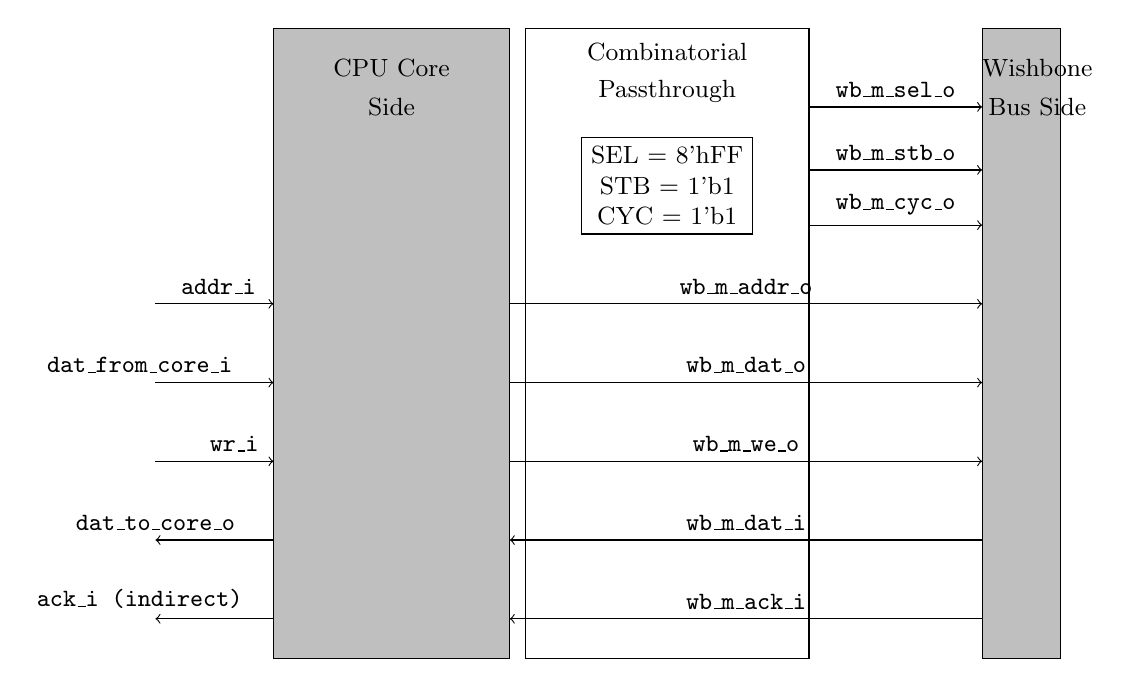
\begin{tikzpicture}
  % CPU/core side (left)
  \filldraw[fill=lightgray, draw=black] (0,0) rectangle (3,8);
  \node[align=center] at (1.5,7.5) {\small CPU Core};
  \node[align=center] at (1.5,7.0) {\small Side};
  % CPU inputs
  \draw[->] (-1.5,4.5) -- (0,4.5) node[left,above,xshift=-0.7cm]{\small \texttt{addr\_i}};
  \draw[->] (-1.5,3.5) -- (0,3.5) node[left,above,xshift=-1.7cm]{\small \texttt{dat\_from\_core\_i}};
  \draw[->] (-1.5,2.5) -- (0,2.5) node[left,above,xshift=-0.5cm]{\small \texttt{wr\_i}};
  \draw[<-] (-1.5,1.5) -- (0,1.5) node[left,above,xshift=-1.5cm]{\small \texttt{dat\_to\_core\_o}};
  \draw[<-] (-1.5,0.5) -- (0,0.5) node[left,above,xshift=-1.7cm]{\small \texttt{ack\_i (indirect)}};
  % Passthrough box (centre)
  \filldraw[fill=white, draw=black] (3.2,0.0) rectangle (6.8,8.0);
  \node[align=center] at (5,7.7) {\small Combinatorial};
  \node[align=center] at (5,7.2) {\small Passthrough};
  \node[draw,fill=white,align=center,font=\small] at (5,6.0)
    {SEL = 8'hFF \\ STB = 1'b1 \\ CYC = 1'b1};
  % Wishbone side (right)
  \filldraw[fill=lightgray, draw=black] (9,0) rectangle (10,8);
  \node[align=center] at (9.7,7.5) {\small Wishbone};
  \node[align=center] at (9.7,7.0) {\small Bus Side};
  % passthrough outputs
  \draw[->] (3,4.5) -- (9,4.5) node[midway,above]{\small \texttt{wb\_m\_addr\_o}};
  \draw[->] (3,3.5) -- (9,3.5) node[midway,above]{\small \texttt{wb\_m\_dat\_o}};
  \draw[->] (3,2.5) -- (9,2.5) node[midway,above]{\small \texttt{wb\_m\_we\_o}};
  \draw[<-] (3,1.5) -- (9,1.5) node[midway,above]{\small \texttt{wb\_m\_dat\_i}};
  \draw[<-] (3,0.5) -- (9,0.5) node[midway,above]{\small \texttt{wb\_m\_ack\_i}};
  % constant signals from logic box
  \draw[->] (6.8,7.0) -- (9,7.0) node[midway,above]{\small \texttt{wb\_m\_sel\_o}};
  \draw[->] (6.8,6.2) -- (9,6.2) node[midway,above]{\small \texttt{wb\_m\_stb\_o}};
  \draw[->] (6.8,5.5) -- (9,5.5) node[midway,above]{\small \texttt{wb\_m\_cyc\_o}};
\end{tikzpicture}
\caption{as\_master\_bpi -- Internal Signal Flow}
\label{fig:asMasterBpi01}
\end{figure}

Table~\ref{tab:asMasterBpiInt} lists the internal signals (none in this
implementation, as the module is purely combinatorial):

\begin{table}[H]
\caption{as\_master\_bpi Internal Signals}
\label{tab:asMasterBpiInt}
\centering
\begin{tabularx}{\textwidth}{|l |l |l |X|}
  \hline
  Signal & Type & Width & Description \\
  \hline
  \hline
  (none) & -- & -- & All logic is combinatorial; no internal signals \\
  \hline
\end{tabularx}
\end{table}

\subsubsection{Instantiation}

\begin{verbatim}
as_master_bpi #(
    .addr_width ( 64 ),
    .data_width ( 64 )
) u_cpu_bpi (
    .rst_i              ( rst_i              ),
    .clk_i              ( clk_i              ),
    // CPU core side
    .addr_i             ( cpu_addr_s         ),
    .dat_from_core_i    ( cpu_wdat_s         ),
    .dat_to_core_o      ( cpu_rdat_s         ),
    .wr_i               ( cpu_wr_s           ),
    // wishbone side
    .wb_m_addr_o        ( wb_m_addr_s        ),
    .wb_m_dat_i         ( wb_m_dat_i_s       ),
    .wb_m_dat_o         ( wb_m_dat_o_s       ),
    .wb_m_we_o          ( wb_m_we_s          ),
    .wb_m_sel_o         ( wb_m_sel_s         ),
    .wb_m_stb_o         ( wb_m_stb_s         ),
    .wb_m_ack_i         ( wb_m_ack_s         ),
    .wb_m_cyc_o         ( wb_m_cyc_s         )
);
\end{verbatim}

\subsubsection{Limitations and Design Rules}

\begin{itemize}
  \item \textbf{Continuous bus occupation.}
    Because \texttt{STB} and \texttt{CYC} are permanently asserted,
    the master occupies the bus at all times.
    Multi-master arbitration requires that these signals are gated
    by the arbiter before being placed on the shared bus.
  \item \textbf{No idle state.}
    The master BPI does not support idle cycles between transfers.
    The surrounding CPU core logic must insert idle cycles if needed
    by controlling \texttt{addr\_i} and \texttt{wr\_i} appropriately and
    ignoring any ACK responses during idle periods.
  \item \textbf{ACK not evaluated.}
    \texttt{wb\_m\_ack\_i} is an input of the BPI but is not used and not
    passed on to the CPU. All slaves must therefore be zero-wait-state
    (see Functional Overview above).
  \item \textbf{No error handling.}
    There is no support for Wishbone \texttt{ERR\_I} or \texttt{RTY\_I}.
\end{itemize}


%%%%%%%%%%%%%%%%%%%%%%%%%%%%%%%%%%%%%%%%%%%%%%%%%%%%%%%%%%%%%%%%%%%%%%%%%%%%%
\subsection{Bus Interconnect}
\label{subsec:asBusInterconnect}
%%%%%%%%%%%%%%%%%%%%%%%%%%%%%%%%%%%%%%%%%%%%%%%%%%%%%%%%%%%%%%%%%%%%%%%%%%%%%

\subsubsection{Wishbone Address Map}

Each Wishbone slave is mapped to a contiguous, non-overlapping region of
the address space. The address decoder \texttt{as\_decode} generates one
chip select per region; \texttt{STB} is forwarded only to the selected
slave. The read data multiplexer selects the slave by chip select and returns 0
if no slave is selected. The address boundaries are defined in
Table~\ref{tab:sysmap}.

\subsubsection{Wishbone Topology}

The Wishbone implementation uses a \textbf{shared bus} topology with a single
master (the CPU core). A crossbar switch is not implemented because there is
only one Wishbone master and the zero-wait-state slave design means bus
bandwidth is limited only by the clock frequency.

\subsubsection{Peripheral Register Offset Alignment}

All peripheral registers are 64\,bit wide and aligned to 8-byte boundaries.
The address offset within a peripheral starts at \texttt{0x00} for the
ID register and increases in steps of \texttt{0x08}.
This is consistent with the Wishbone bus data width and the 64-bit
alignment of the RISC-V load and store instructions used to access the
peripheral registers.

\subsubsection{Read-Modify-Write}

The Wishbone protocol as implemented does not support atomic
read-modify-write operations.
Software must therefore use disable-interrupt / critical-section
patterns when accessing shared registers from multiple contexts.
